\documentclass[12pt]{article}

\usepackage[margin=1in]{geometry}
\usepackage{amsmath,amsthm,amssymb,graphicx,gensymb,multicol,mathtools}
\usepackage{xspace}
\usepackage{color}
\usepackage{alltt}
\usepackage[english]{babel}
\usepackage[autostyle, english = american]{csquotes}
\usepackage{braket}
\usepackage{tikz, pgfplots}
\usepackage[T1]{fontenc}   % so _, <, and > print correctly in text.
\usepackage{biblatex}
\usepackage[strings]{underscore}    % to use "_" in text
\usepackage{hyperref}  % Must be last package
\hypersetup{
  colorlinks=true,
  linkcolor=blue,
  filecolor=red,
  urlcolor=cyan,
}

\MakeOuterQuote{"}
\graphicspath{{figures/}}
\pgfplotsset{compat=newest}
\allowdisplaybreaks

\addbibresource{bibfile.bib}

\newcommand{\pp}{\mathbf{p}}
\newcommand{\uu}{\mathbf{u}}
\newcommand{\vv}{\mathbf{v}}
\newcommand{\ww}{\mathbf{w}}
\newcommand{\xx}{\mathbf{\hat{x}}}
\newcommand{\yy}{\mathbf{\hat{y}}}
\newcommand{\zz}{\mathbf{\hat{z}}}
\newcommand{\rr}{\mathbf{\hat{r}}}
\newcommand{\rrr}{\mathbf{r}}
\newcommand{\ppp}{\mathbf{p}}
\newcommand{\xxx}{\mathbf{x}}
\newcommand{\nnot}{\sim \!}
\let\oldemptyset\emptyset
\let\emptyset\varnothing

%for QM:
\newcommand{\intii}{\int_{-\infty}^\infty}
\newcommand{\intoi}{\int_0^\infty}
\newcommand{\HH}{\mathbb{H}}
\newcommand{\ang}[3]{\,^{#1} {#2}_{#3}}
\newcommand{\tr}{\mathrm{Tr}}

%units:
\newcommand{\s}{\, \mathrm{s}}
\newcommand{\m}{\, \mathrm{m}}
\newcommand{\eV}{\, \mathrm{eV}}
\newcommand{\MeV}{\, \mathrm{MeV}}
\newcommand{\ly}{\, \mathrm{ly}}
\newcommand{\dxds}{\frac{dx}{ds}}
\newcommand{\dyds}{\frac{dy}{ds}}
\newcommand{\dxdsmin}{\dxds_{\mathrm{min}}}
\newcommand{\dxdsmax}{\dxds_{\mathrm{max}}}
\newcommand{\dydsmax}{\left| \dyds \right|_{\mathrm{max}}}
\newcommand{\exes}{\texttt{converter\_simulation}\xspace}
\newcommand{\exef}{\texttt{converter\_fitter}\xspace}
\newcommand{\configfile}{\texttt{config.txt}\xspace}
\newcommand{\bmad}{\textit{Bmad}\xspace}
\newcommand{\targetm}{\texttt{material}\xspace}
\newcommand{\targett}{\texttt{thicknesses}\xspace}
\newcommand{\pcin}{\texttt{pc\_in}\xspace}
\newcommand{\outpcmin}{\texttt{out\_pc\_min}\xspace}
\newcommand{\outpcmax}{\texttt{out\_pc\_max}\xspace}
\newcommand{\dxydsmax}{\texttt{dxy\_ds\_max}\xspace}
\newcommand{\outdir}{\texttt{output\_directory}\xspace}
%\newcommand{\numbins}{\texttt{num\_bins}\xspace}
\newcommand{\numrbins}{\texttt{num\_r\_bins}\xspace}
\newcommand{\numpcbins}{\texttt{num\_pc\_bins}\xspace}
\newcommand{\fitxpt}{\texttt{fit\_crossover}\xspace}
\newcommand{\B}{$\backslash$}

\newenvironment{example}
  {\vspace{-2.5ex} \begin{alltt}}
  {\end{alltt} \vspace{-2.2ex}}

\newenvironment{problem}[2][Problem]{\begin{trivlist}
\item[\hskip \labelsep {\bfseries #1}\hskip \labelsep {\bfseries #2.}]}{\end{trivlist}}

\setlength{\parskip}{1.5ex}
\setlength{\parindent}{0ex}

%----------------------------------

\begin{document}

\title{Bmad Converter Model}
\author{John Mastroberti}

\maketitle

\tableofcontents

\newpage

\section{Introduction}

This monograph discusses the converter model used in converter lattice elements in \bmad. In a
converter, incoming particles generate particles of a different type. For example, a converter may
be used to simulate the production of positrons produced when a tungsten target plate is bombarded
by electrons.

The converter model currently in \bmad discussed here replaces an older model that was developed by
Daniel Fromowitz\cite{b:fromowitz}. This older model used equations to model the output
distribution.  The problems with this approach were the approximations that were used in developing
the equations coupled with uncertainty as to how to calculate the various coefficients that were
needed if parameters like the target material or the species of particles simulated were varied.

The present model replaces the equations of the older model with probability distribution tables for
the energy and radial distribution of the outgoing particle along with a generalized
parameterization of the probability distribution of the outgoing particles's direction of
propagation.  Probability distribution table values and coefficients needed to characterize the
velocity distribution are obtained through a Geant\cite{geant} simulation. These tables and
coefficients can then be stored in a \bmad lattice file and used for efficient generation of
outgoing particles. The present model is not only more accurate but can also simulate a wider range
of parameters in terms of converter thickness, converter material, incoming particle energy, and
different particle species.

While it would be technically feasible to use Geant directly to simulate the converter process, the
production of outgoing particles in the converter is a stochastic process, the details of which are
computationally expensive. The use of probability distribution tables, which only have to be
computed once, while not as accurate, speeds up the computation time by orders of magnitude.

The imputus for developing the new model was to better simulate the converter in the Cornell CESR
Linac which generated positrons due to bombardment of a tungsten plate by electrons. The electrons
have an energy of order $\sim 100 \MeV$.  As the incident electrons pass through the
converter, they emit photons via Bremsstrahlung, which in turn decay to $e^+ e^-$ pairs:
\begin{align}
  e^- + Z \rightarrow e^- + Z + \gamma \rightarrow e^- + Z + e^+ + e^-
\end{align}

%-------------------------------------------------------------
\newpage
\section{The converter model}

The probability distribution is computed assuming assuming that the incoming particle's momentum is
perpendicular to the surface of the converter. This is reasonable since deviations of the
probability distribution will be second order in the transverse momentum. The coordinate system is
shown in Figure \ref{fig:coords}.
\begin{figure}
\centering
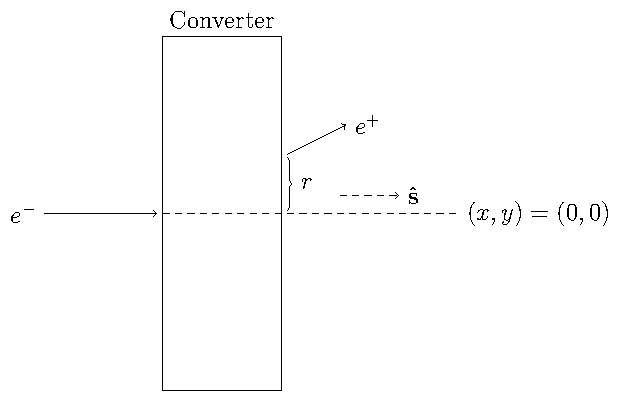
\includegraphics[width=0.6\textwidth]{coords1.pdf}
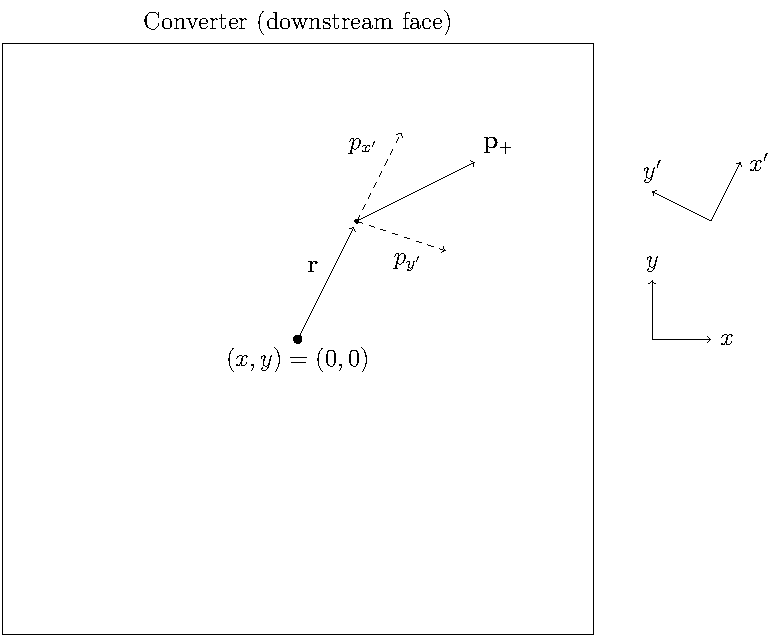
\includegraphics[width=0.8\textwidth]{coords2.pdf}
\caption{Coordinates used to describe the outgoing particles exiting the converter. The incoming particle is
labeled $e^-$ and the outging particle is labeled $e^+$.}
\label{fig:coords}
\end{figure}
The outgoing particle's position on the downstream face of the converter is then described by $r$,
its distance from the $z$ axis, and the angle $\theta$ shown in the figure. By symmetry, $\theta$
must be distributed uniformly between $0$ and $2\pi$ and so the probability distributions will be
independent of $\theta$. The $x$-axis is defined to be in the same direction as $\rrr$. The
$y$-axis is choisen such that $(x,y,z)$ is a right handed orthogonal coordinate system.

\subsection{Probability Distributions}

The incoming particle is labeled by a plus symbol subscript and the outgoing particle is labeled by
a minus symbol subscript. The outgoing particle as it leaves the surface of the converter is
characterized by $\theta$, its momentum $p_+$, the offset from the origin $r$, and the $dx/ds$ and
$dy/ds$ slopes with
\begin{align}
p_+ c & = \left| \mathbf{p}_+ \right| c \\
\dxds & = \frac{p_x}{p_s} \\
\dyds & = \frac{p_y}{p_s}
\end{align}
Ignoring $\theta$, we seek the distribution
\begin{align}
P \left( p_+ c, r, \dxds, \dyds \right)
\end{align}
which describes the probability that an outgoing particle will attain particular values of $p_+ c$,
$r$, $\dxds$, and $\dyds$. This probability distribution is dependent upon the incoming particle's
energy $p_- c$, as well as the thickness $T$ and material type of the converter. This will be discussed later.

$P$ is normalized to the number of outgoing particles produced per incoming particle:
\begin{align}
\int P \left( p_+ c, r, \dxds, \dyds \right) \, d(p_+ c) \, dr \, d \! \left( \dxds \right) d \! \left( \dyds \right) & = \frac{N_+}{N_-}
\end{align}
This normalization lets us easily account for the fact that number of outgoing particles produced
varies with the incoming particle energy and converter thickness. $P$ can be decomposed into two distributions:
\begin{align}
P \left( p_+ c, r, \dxds, \dyds \right) & = P_1 \left( p_+ c, r \right) P_2 \left( \dxds, \dyds ; p_+ c , r \right),
\end{align}
where $P_1$ is choisen to be normalized to $N_+/N_-$ and $P_2$ is normalized to 1.

\subsection{$P_1$ and $P_2$ Parameterization}

Using Geant\cite{geant}, A number of incoming particles of a given energy incident upon a converter
of a given thickness is simulated.  The values of $p_+ c$, $r$, $\dxds$, and $\dyds$ for each
outgoing particle at the downstream face of the converter is recorded. This data is then binned into
a two-dimensional histogram by $p_+ c$ and $r$. The sizes of the bins are chosen non-uniformly so
that each bin holds approximately the same number of outgoing particles. The binned data produces a
probability distribution table that characterizes $P_1(p_+c, r)$.

To model $P_2$, for each $(p_+ c, r)$ bin, the distribution of particles in $dx/ds$ and $dy/ds$ is
fit to the functional form
\begin{align}
P_2 \left( \dxds, \dyds; p_+ c, r \right) & = A \frac{1 + \beta \dxds}{1 + \alpha_x^2 \left( \dxds - c_x \right)^2 + \alpha_y^2 \left( \dyds \right)^2}. \label{eq:cauchy}
\end{align}
Since $P_2$ is normalized to $1$, $A$ is not a true fit parameter, but is fixed by the
normalization.  The fit gives values of $c_x$, $\alpha_x$, $\alpha_y$, and $\beta$ in each $(p_+ c,
r)$ bin.  The distribution of $\dxds$ and $\dyds$ is also characterized by $\dxds_{min}$,
$\dxds_{max}$ and $\left| \dyds \right|_{max}$, which define the rectangle in $\dxds \times \dyds$
space where $P_2 \left( \dxds, \dyds \right)$ is significantly nonzero.  Fits to each of the
parameters $c_x, \alpha_x, \alpha_y, \beta, \dxds_{min}, \dxds_{max}, \left| \dyds_{max} \right|$ as
functions of $p_+ c$ and $r$ are made as follows:
\begin{itemize}
\item
At each value of $p_+ c$ below a user-defined cutoff, a 1D fit is performed using the form
\begin{align}
\pi(r) = a_0 + a_1 r+ a_2 r^2 + a_3 r^3 + a_4 r^4 \label{eq:fit1}
\end{align}
for each parameter $\pi =c_x, \alpha_x, \alpha_y, \beta, \dxdsmin, \dxdsmax, \dydsmax$.  For $c_x$
and $\beta$, $a_0$ is fixed to be 0, as $c_x$ and $\beta$ must be zero at $r=0$ by symmetry.  For
all other parameters, $a_4$ is fixed to be zero, so that a third degree polynomial is fit instead of
a fourth degree polynomial.

\item
Above the user-defined $p_+ c$ cutoff, a 2D fit is performed using the form
\begin{align}
\pi(r) = (1 + a_1 (p_+c) + a_2 (p_+c)^2 + a_3 (p_+c)^3)
         (b_0 + b_1 r + b_2 r^2 + b_3 r^3) e^{-(k_p (p_+ c) + k_r r)} + C \label{eq:fit2}
\end{align}
for each parameter $\pi =c_x, \alpha_x, \alpha_y, \beta, \dxdsmin, \dxdsmax, \dydsmax$.  The
parameter $C$ is only used for $\dxdsmin$.  Note that the constant term for the $p_+ c$
polynomial is set to $1$ in each case.  This must be done so that the fitting problem is non-degenerate.

\end{itemize}
These fits give an approximation of $P_2 \left( \dxds, \dyds; p_+ c, r \right)$.

%-------------------------------------------------------------
\newpage
\section{Setup for Generating the Probability Parameters}

Generating the probability parameters has two main stages. In the first stage, the particle creation
events are simulated with Geant, and the resulting outgoing particles are binned into a
histogram. In the second stage, fits are performed for $\dxds$ and $\dyds$.  Each stage has an
associated executable: \exes for the first stage, and \exef for the second.

After the probability parameters are generated, a \bmad lattice file can be created that contains
these parameters and this lattice file is used for simulating the converter independent of Geant.

\subsection{Dependencies}
\label{s:deps}

Builds require a C++ compiler with support for C++17. GCC 8 or higher should be fine.

A built \bmad Distribution or Release is a prerequisite. See the \bmad web pages (or your local
\bmad Guru) for details.

Needed is an up to date installation of Geant4 on your system. See the Geant4 installation guide
below for details on how to get Geant4 up and running on Linux.  You will also need \texttt{cmake}
version 3.8 or greater installed.

\subsection{Geant4 Installation Guide}

This guide is an abbreviated version of the instructions found on
\href{http://geant4-userdoc.web.cern.ch/geant4-userdoc/UsersGuides/InstallationGuide/html/}{the
Geant4 website}.
\begin{enumerate}
\item
Create a directory, here called \texttt{GEANT_DIR}, where Geant will be installed and \texttt{cd}
to this directory.

\item
Download the .tar.gz source files archive from \url{https://geant4.web.cern.ch/support/download}
into \texttt{GEANT_DIR} and unpack with
\begin{example}
  tar xzvf geant4.10.06.tar.gz
\end{example}
Change the version number as appropriate. There should now be a directory \texttt{geant4.10.06}.

\item
Make a sub-directory where you will build Geant with
\begin{example}
  mkdir geant-build
\end{example}

\item
\texttt{cd} to this new directory, and use \texttt{cmake} to configure the Geant4 build with
\begin{example}
  cmake -DGEANT4_INSTALL_DATA=ON -DGEANT4_BUILD_MULTITHREADED=ON \B
        -DCMAKE_INSTALL_PREFIX=$GEANT_DIR/geant4-build \B
        ../geant4.10.06
\end{example}
Change the version number as appropriate. The \texttt{GEANT4_INSTALL_DATA} flag will cause the
necessary data sets to be downloaded when Geant is built, and the \texttt{CMAKE_INSTALL_PREFIX} flag
sets the install directory. The \texttt{GEANT4_BUILD_MULTITHREADED} causes Geant to be run
multithreaded. Remove this flag to run single threaded. Due to the substantial associated
performance improvement, it is highly recommended that Geant be compiled for multithreaded use.

Note: if you encounter the the error
\begin{example}
  Could NOT find EXPAT (missing: EXPAT_LIBRARY EXPAT_INCLUDE_DIR)
\end{example}
at this step, try editting the file
\begin{example}
  ../geant4.10.06/cmake/Modules/Geant4OptionalComponentents.cmake
\end{example}
replacing the line
\begin{example}
  option(GEANT4_USE_SYSTEM_EXPAT "Use system Expat library" ON)
\end{example}
with
\begin{example}
  option(GEANT4_USE_SYSTEM_EXPAT "Use system Expat library" OFF)
\end{example}
and then re-run the above \texttt{cmake} command.

\item
After \texttt{cmake} finished running, start building Geant with
\begin{example}
  make -j4
\end{example}
This will run four threads. You can change the number of threads to increase or decrease the compile
speed.

\item
Once the compilation has finished, install with
\begin{example}
  make install
\end{example}
\end{enumerate}

%--------------------------------

\subsection{Compiling the Executables} The converter simulation and fitting programs are distributed
as part of any \bmad Distribution or Release and are located in the \texttt{util\_programs}
directory. [If you are not sure where your Distribution or Release is, ask you local \bmad Guru.]
You may need to make a local copy of the \texttt{util\_programs} directory if you do not have write
access to the Distribution or Release version. This can be done with the command:
\begin{example}
  svn co https://accserv.lepp.cornell.edu/svn/trunk/src/util_programs
\end{example}

The file \texttt{\$GEANT_DIR/geant-build/geant4make.sh} must be sourced to add Geant4 to your path.
To do so, use the following commands:
\begin{example}
  cd $GEANT_DIR/geant-build 
  source geant4make.sh
\end{example}

Also execute the command
\begin{example}
  export ACC_BUILD_TEST_EXES="Y"
\end{example}

Now \texttt{cd} to the \texttt{util\_programs} folder, and then simply run \texttt{mk} to build
\exes and \exef. If you get errors like:
\begin{example}
  util_programs/converter_element_modeling/fitter/cauchy.cpp:35:10:
  error: expected unqualified-id before '[' token
      auto [xval, yval, binval] = bins[i];
           ^
\end{example}
The problem is that the C++ compiler does not support C++17.

If \texttt{ROOT} is the name of the directory containing the \texttt{util_programs} directory, the
executables will be in the directory
\begin{example}
  $ROOT/production/bin
\end{example}

Note that if Geant is ever recompiled (for example, to enable multithreaded support),
\exes will also need to be recompiled.

%-------------------------------------------------------------
\newpage
\section{How to run the programs}

\subsection{Configuration} Both \exes and \exef are configured by editing the file \configfile,
which should be in the working directory where you run both executables.  Each line in this file
should have the form
\begin{example}
  setting = value
\end{example}
Comments can be inserted with an exclamation mark \texttt{!} and last until the end of the line.
An example config file, with all available settings listed, is shown below.
\begin{example}
  ! Example configuration file
  ! The ! introduces a comment that lasts until the end of the line
  material = tungsten ! Defines the converter material
  thicknesses = 6.35 mm, 1.0 cm ! Defines the target thicknesses to be simulated
  pc_in = 300 MeV, 500 MeV, 1 GeV ! Defines the incoming particle
                                  ! energies to be simulated
  out_pc_min = 0 ! Minimum pc cutoff for outgoing particles, defaults to 0
  out_pc_max = 100000000 ! Maximum pc cutoff for outgoing particles (in eV here)
  dxy_ds_max = 10 ! Maximum cutoff for the magnitude of dx/ds
                  ! and dy/ds allowed for outgoing particles
  output_directory = sim_data ! Name of the directory where data will be output,
                              ! should be specified relative to the working directory
                              ! Defaults to sim_data
  num_pc_bins = 12 ! Number of pc bins to use for histogram binning
  num_r_bins = 20 ! Number of r bins to use for histogram binning
  fit_crossover = 10 MeV ! For alpha and beta fits, this defines the
                         ! point where the fitter transitions from 1D
                         ! to 2D fits, defaults to 10 MeV
\end{example}

All settings accept a single value, except for \pcin and \targett, which accept a comma separated
list of values.  The settings \outpcmin, \outdir, and \fitxpt have default values, while
the settings \targetm, \targett, \pcin, \outpcmax, \numpcbins, \numrbins, and \dxydsmax must be specified in the file.

The settings \pcin, \outpcmin, and \outpcmax take values with dimensions of energy.  These default
to eV if no unit is specified, although \texttt{MeV} and \texttt{GeV} can be added as suffixes to
use MeV and GeV instead as shown in the sample file.  The \targett setting takes values with
dimensions of length.  The default unit is meters, although \texttt{cm} and \texttt{mm} are
supported as well.

The settings \numpcbins and \numrbins control the number of bins used in the histogram.
Both values must be set in the config file.

\subsection{The Simulation Program}

To run \exes and perform the converter simulation, first create and edit the configuration file
\configfile, and place it in your working directory.  Then, just run
\begin{example}
  $ROOT/production/bin/converter_simulation
\end{example}
where \texttt{ROOT} is the directory containing the \texttt{util_programs} directory. The program will
parse your config file and report the settings it read, and report if there are any problems reading
your config file.  It will then verify that the directory you set for \outdir does not exist or is
empty, and will ask you if you want to overwrite it if it already exists.  Then, for each value of
\pcin and \targett specified in the config file, the program will simulate many particle creation
events for those settings.  For example, with the above config file, six simulations will be run
with the following settings:
\begin{itemize}
\item $p_- c = 300$ MeV  and $T = 6.35$ mm
\item $p_- c = 500$ MeV  and $T = 6.35$ mm
\item $p_- c = 1$   GeV  and $T = 6.35$ mm
\item $p_- c = 300$ MeV  and $T = 1$    cm
\item $p_- c = 500$ MeV  and $T = 1$    cm
\item $p_- c = 1$   GeV  and $T = 1$    cm
\end{itemize}
Depending on your computer and the number of different simulations that need to be run, this step
may take several hours.
%Fortunately, this only has to be done once to set up the \bmad  converter element.


\subsection{The Fitting Program}

Once the simulations are complete, just run
\begin{example}
  $ROOT/production/bin/converter_fitter
\end{example}
in the same directory where you ran \exes.  \exef will re-parse your config file for the settings it
needs, and will again report on any errors it encounters.  It then performs the fit from Equation
\ref{eq:cauchy} in each of the $(p_+c, r)$ bins for each simulation.  At this stage, the program may
report that the fitting iteration limit has been reached a few times; this is not cause for concern.
Once this step is complete, and the program has obtained values of $c_x$, $\alpha_x$, $\alpha_y$,
and $\beta$ in each $(p_+c, r)$ bin, it performs the fits from Equations \ref{eq:fit1}-\ref{eq:fit2}
on these fit parameters.  Finally, the results of the simulation, as well as the results of the
fits, are output to the file \texttt{converter.bmad}, located in the \outdir specified in the config
file.

%-------------------------------------------------------------
\newpage
\section{Output from the Programs}

\subsection{Simulation Output}

After running the \exes program, the directory specified by the \texttt{output\_directory} setting
in the configuration file will exist in your working directory.  Inside it, there will be one file
of the format '\texttt{E\{pc\_in\}\_T\{thickness\}\_er.dat}', for each incoming $p_- c$ and target
thickness specified in the configuration file, where \texttt{pc\_in} and \texttt{thickness} are the
$p_- c$ and thickness in MeV and cm respectively.  These files contained the binned data which
approximate $P_1(p_+ c, r)$.  The output directory will also contain a directory \texttt{dir\_dat},
with subdirectories \texttt{E\{pc\_in\}\_T\{thickness\}\_er.dat} for each $p_- c$ and target
thickness combination.  Each of these directories will contain files named
\texttt{E\{pc\_out\}\_r\{r\_out\}\_bin.dat}, which contain the binned $\dxds$ and $\dyds$ data used
by \exef.

\subsection{Fitting Output}

After running the \exef program, the output directory will also contain a file called
\texttt{converter.bmad}.  This file aggregates all the information about $P_1$ and $P_2$ at each
$p_+ c$ and target thickness tested, and is designed for use with a \bmad converter element.

\subsubsection{Gnuplot Files}

\exef  also generates several gnuplot scripts for inspecting the quality of the obtained fits.
These are all written to the individual \texttt{E\{\}\_r\{\}} directories under \texttt{dir\_dat}.

Each of the $(p_+ c, r)$ bins gets two gnuplot scripts:
\texttt{cauchy\_E\{pc\_out\}\_r\{r\_out\}.gp} and \texttt{meta\_E\{pc\_out\}\_r\{r\_out\}.gp}.  The
scripts with the \texttt{cauchy} prefix display the distribution $P_2$ obtained by directly fitting
Equation \ref{eq:cauchy} to the data in each bin.  The scripts with the \texttt{meta} prefix display
the distribution $P_2$ obtained from evaluating the fits from Equations \ref{eq:fit1}-\ref{eq:fit2}
to the Cauchy fit parameters.

\exef also outputs scripts for viewing the fits from Equations \ref{eq:fit1}-\ref{eq:fit2} across
all $(p_+ c, r)$ bins.  These are named \texttt{c\_x\_master.gp}, \texttt{a\_x\_master.gp},
\texttt{a\_y\_master.gp}, \texttt{beta\_master.gp}, \texttt{dxds\_min\_master.gp},
\texttt{dxds\_max\_master.gp}, and \texttt{dyds\_max\_master.gp}.

To view any of these plots, simply open Gnuplot in the \texttt{E\{\}\_T\{\}} directory of interest,
and call the script.  For example:
\begin{example}
  > cd /home/user/sim_data/dir_dat/E300_T0.635
  > gnuplot
  gnuplot> call 'c_x_master.gp'
\end{example}
This will open the plot for $c_x$ across all $(p_+ c, r)$ bins for $p_+ c = 300$ MeV, $T = 0.635$ cm.

%-------------------------------------------------------------
\newpage
\section{The \bmad  Converter Element}

As mention in the previous section, \exef outputs a file, \texttt{converter.bmad}, which encodes all
of the simulation and fitting output, and can be used to specify the properties of a \bmad converter
element.  See the \bmad manual for the full details regarding the converter element in \bmad.

The user should be aware that \bmad's method of generating outgoing particles may not be completely
faithful to the simulation results.  In particular, \bmad uses linear interpolation for the
$P_1(p_+c, r)$ distribution.  This can cause noticeable discrepancies on the edges of the
distribution, especially in the bins with the lowest values of $p_+ c$.  Since $P_1(p_+c, r)$
changes rapidly at low $p_+ c$, and \bmad additionally does not generate outgoing particles with
$p_+ c$ lower than the lowest value of $p_+ c$ for the bins, \bmad does not generate as many
outgoing particles at low $p_+ c$ as it should.

\appendix

%-------------------------------------------------------------
\newpage
\section{Notes for ACC Computer Users}

As detailed in Section \ref{s:deps}, building \exes and \exef requires GSL, Geant, and a C++
compiler with support for C++17.  GSL is already available on the lab machines, and a build of Geant
is provided at \texttt{/nfs/acc/temp/jmm699/geant}.  To get access to this Geant build, you can
simply add the following to your \texttt{.bashrc}:
\begin{example}
  cd /nfs/acc/temp/jmm699/geant/geant4.10.06.p01-build 
  source geant4make.sh 
  cd -
\end{example}
As for the C++ compiler, you can get access to GCC 8.3 by adding
\begin{example}
  source /opt/rh/devtoolset-8/enable
\end{example}
to your \texttt{.bashrc}.

\printbibliography

\end{document}
